%Lezione 04

\subsection{Amplificatore operazionale}

Si introduce il modello dell'amplificatore operazionale, rappresentato da un
triangolo con tre morsetti, due in ingresso ed uno in uscita, quello con il
segno $-$ viene detto invertente, quello con il segno $+$ è non invertente.
Solitamente sono anche indicati i morsetti di alimentazione.
\begin{figure}[H]
 \centering
 \begin{circuitikz}
  \draw (0,0) node[op amp, anchor=-](OA){}
 (OA.+) -- ++(-1,0)
 to [short, -*] (-1,-1);
 \draw
(OA.-) -- ++(-1,0)
 to [short, -*] (-1,0);
 \draw (-1,-1) to [open,v^>=$e$] (-1,0);
 \draw (OA.out) -- ++(0,0) to [open,v^<=$v$,*-*] ++(0,-1)
  node[ground]{} ;
  \draw (OA.up)  node[vcc]{$+V_{cc}$};
  \draw (OA.down) node[vee]{$-V_{cc}$};
 \end{circuitikz}
\end{figure}
L'equazione caratteristica è
$$
v = -Ae
$$
Solitamente il valore $A$ è molto grande, anche \SI{e6}{} così come l'impedenza
d'ingresso tra i morsetti $+$ e $-$.

Dato un segnale in ingresso dunque, questo verrà restituito in uscita invertito
ed amplificato. Questa condizione è verificata se si suppone che la $v$ è
compresa tra i valori $[-V_{cc},+V_{cc}]$ di alimentazione.
In caso contrario l'uscita verrebbe ``tagliata'' e ci sarebbe un comportamento
non lineare, ipotesi di lavoro sempre evitata in questo corso.

Di conseguenza il segnale d'ingresso dovrebbe essere di valori pari a $v/A$,
valori bassissimi, si può ritenere dunque che la caduta di tensione
all'ingresso sarà prossima a \SI{0}{\volt}, è quindi come se l'ingresso fosse
un corto circuito (anche se non lo è).

L'impedenza d'ingresso, essendo di ordine elevato, implica che anche la
corrente nello stadio d'ingresso sia prossima a \si{0}, quindi si può modellare
come un circuito aperto.

In conclusione lo stadio d'ingresso si comporta sia da circuito chiuso che
circuito aperto e viene chiamato \textbf{corto circuito virtuale}.

Lo stadio d'uscita è confrontabile con un generatore ideale di tensione.

Si consideri il seguente circuito:
\begin{figure}[H]
\centering
\begin{circuitikz}
\draw (3,-.5) node[op amp](op){}
      (0,0) to [R=$R_1$,i=$i$,*-*]  (op.-)
            to ++(0,1)
            to [R=$R_2$,i>^=$i$] (4,1);
\draw (op.out) |- (4,1) ;
\draw (op.out) to [short,-*] ++(1,0)
                to [open,-*,v^<=$v$] ++(0,-0.5)
                node[ground]{};
\draw (op.+) to [short] ++(0,-.5)
        node[ground]{};
\draw (0,-1.5) node[ground]{} to [open,v^>=$e$,*-*] (0,0);
\end{circuitikz}
\end{figure}

Si ricorda che la tensione ai capi dell'ingressodell'amplificatore è nulla e la
corrente in ingresso lo è altrettanto.

Se si considera la maglia composta dal morsetto di uscita, la resistenza $R_2$
e il morsetto di ingresso si ottiene che la tensione ai capi di $R_2$ è pari a
$v$ ossia $v = -R_2i$.

Analogamente allo stadio d'ingresso, la tensione ai capi di $R_1$ è pari ad $e$
ossia $e = R_1i$.

Le due resistenze sono dunque attraversate dalla stessa corrente $i$.

Sostituendo le due equazioni precedenti si ottiene la tensione in uscita in
funzione di quella in ingresso
\begin{equation}
v = -R_2 i = -\frac{R_2}{R_1}e
\label{eq.:amplificatoreOperazionale}
\end{equation}

Si può variare dunque il guadagno dell'amplificatore variando opportunamente il
rapporto tra le resistenze.
Collegando un secondo amplificatore in cascata con guadagno $-1$ si ottiene una
tensione finale concorde a quella in ingresso. Questo secondo elemento viene
definito \textit{buffer}.
Il \textit{buffer} è molto utile per disaccoppiare i circuiti.

\subsection{Circuito integratore}
Si analizza il seguente circuito
\begin{figure}[H]
\centering
\begin{circuitikz}
\draw (3,-.5) node[op amp](op){}
      (0,0) to [R=$R$,i=$i$,*-*]  (op.-)
            to ++(0,1)
            to [C=$C$,i>^=$i$,v<=$v_C$] (4,1);
\draw (op.out) |- (4,1) ;
\draw (op.out) to [short,-*] ++(1,0)
                to [open,-*,v^<=$v$] ++(0,-0.5)
                node[ground]{};
\draw (op.+) to [short] ++(0,-.5)
        node[ground]{};
\draw (0,-1.5) node[ground]{} to [open,v^>=$e$,*-*] (0,0);
\end{circuitikz}
\end{figure}
A differenza del circuito precedente il sistema è dinamico, se ne ricava di
seguito la ISU.

Equazioni caratteristiche
\begin{equation}\left\{\begin{aligned}
v &= -v_C \\
i &= \frac{e}{R} = C \dot{v}_C
\end{aligned}\right.\Rightarrow
e=-RC\dot{v}
\label{eq.:differenzialeIntegratore}
\end{equation}

Si analizzano le variabili seguendo la regola di causalità

$$
\begin{matrix}
 e    & v \\
 (0)  &(1) \\
 u    & x
 \end{matrix}
$$

L'ordine del sistema è unitario dunque il modello ISU non sarà un'equazione
matriciale
$$
\left\{\begin{aligned}
        \dot{x} &= \dot{v} = -\frac{1}{RC} u \\
        y & = v = x
       \end{aligned}\right.
$$
Il sistema è lineare tempo invariante strettamente causale (o proprio LTISP).
Se si integra la \ref{eq.:differenzialeIntegratore} si ottiene
$$
v(t) = v(t_0) - \frac{1}{RC}\int_{t_0}^{t} e(\tau)d\tau
$$
Ossia l'uscita, a meno di un fattore di guadagno è l'integrale dell'ingresso,
si è realizzato un circuito integratore ideale.

\subsubsection{Circuito integratore reale}
Si inserisce in parallelo alla capacità del circuito precedente una resistenza
di scarica parassita $R_s$.

\begin{figure}[H]
\centering
\begin{circuitikz}[smallR/.style={R, resistors/scale=0.5}]
\draw (3,-.5) node[op amp](op){}
      (0,0) to [R=$R$,i=$i$,*-*]  (op.-)
            to ++(0,1)
            to [C=$C$,i>^=$i_C$,v<=$v_C$] (4,1)
            -- ++(0,1) to [smallR,l_=$R_s$,i_<=$i_{R_s}$] ++(-2.1,0) -|
++(0,-1);
\draw (op.out) |- (4,1) ;
\draw (op.out) to [short,-*] ++(1,0)
                to [open,-*,v^<=$v$] ++(0,-0.5)
                node[ground]{};
\draw (op.+) to [short] ++(0,-.5)
        node[ground]{};
\draw (0,-1.5) node[ground]{} to [open,v^>=$e$,*-*] (0,0);
\end{circuitikz}
\end{figure}

Le equazioni del sistema saranno
$$\left\{\begin{aligned}
          v &= -v_C \\
          i &= \frac{e}{R} = C\dot{v}_C + \frac{v_C}{R_s}
         \end{aligned}\right.\Rightarrow
e = -RC\dot{v} - \frac{R}{R_s}v
$$
Si riscrivono le variabili
$$
\begin{matrix}
 e    & v \\
 (0)  &(1) \\
 u    & x
 \end{matrix}
$$
la ISU
$$\left\{\begin{aligned}
\dot{x} &= \frac{1}{R_sC}x - \frac{1}{RC}e\\
y & = v = x
\end{aligned}\right.
$$
È presente un termine aggiuntivo rispetto al precedente sistema.
Se $R_s$ fosse una vera capacità parassita, ossia molto più grande di $R$, si
trascurerebbe il primo termine dell'equazione ritornando al caso precedente; in
caso contrario si è in presenza di un integratore \textit{reale}, governato
ossia da una costante di tempo che ne indica la velocità di scarica.

\newpage
\subsection{Circuito derivatore}
Si invertono in questo circuito la posizione del condensatore e della
resistenza, si suppone inoltre di alimentare il circuito con un generatore
ideale di tensione.
\begin{figure}[H]
\centering
\begin{circuitikz}
\draw (3,-.5) node[op amp](op){}
      (0,0) to [C=$C$,i=$i$,v_<=$e$,*-*]  (op.-)
            to ++(0,1)
            to [R=$R$,i>^=$i$,v<=$v_R$] (4,1);
\draw (op.out) |- (4,1) ;
\draw (op.out) to [short,-*] ++(1,0)
                to [open,-*,v^<=$v$] ++(0,-0.5)
                node[ground]{};
\draw (op.+) to [short] ++(0,-.5)
        node[ground]{};
\draw (0,-1.5) node[ground]{} to [open,v^>=$e$,*-*] (0,0);
\end{circuitikz}
\end{figure}

Si scrivono le equazioni
$$
v = -Ri = -RC \dot{e}
$$
il circuito è un derivatore ideale.
In questo caso ideale, il sistema è non causale, dovrebbe fornire in uscita la
derivata del segnale in ingresso.

Sviluppando l'analisi
$$
\dot{e} = -\frac{1}{RC}v
$$
$$
\begin{matrix}
 \dot{e} & v\\
 (1) & (0)
\end{matrix}
$$
seguendo le regole precedenti si direbbe che la variabile causa è la $v$ mentre
l'effetto è la $e$, ciò è in contrasto con l'evidenza fisica del sistema.

La regola di Cauchy non vale per i sistemi non causali.
Si sta affermando che il generatore possa pilotare istantaneamente una capacità.

Per modellare un sistema analogo va inserita nel circuito una resistenza $R_s$
in serie al generatore di tensione (o analogamente alla porta d'ingresso).
\begin{figure}[H]
\centering
\begin{circuitikz}[smallR/.style={R, resistors/scale=0.5}]
\draw (3,-.5) node[op amp](op){}
      (-2,0) to [smallR,l=$R_s$] ++(2,0) to [C=$C$,i=$i$,v_<=$v_C$,*-*]  (op.-)
            to ++(0,1)
            to [R=$R$,i>^=$i$,v<=$v_R$] (4,1);
\draw (op.out) |- (4,1) ;
\draw (op.out) to [short,-*] ++(1,0)
                to [open,-*,v^<=$v$] ++(0,-0.5)
                node[ground]{};
\draw (op.+) to [short] ++(0,-.5)
        node[ground]{};
\draw (-2,-1.5) node[ground]{} to [open,v^>=$e$,*-*] (-2,0);
\end{circuitikz}
\end{figure}
Le equazioni del sistema:
$$\left\{\begin{aligned}
v &= -Ri = -RC\dot{v}_C\\
e &= R_s i + v_C \Rightarrow i = \frac{e-v_C}{R_s}
\end{aligned}\right.$$

Ricavando la $i$ dalla seconda e sostituendo nella prima
$$
\dot{v}_C =
\frac{1}{\cancel{R}C}\left(\frac{\cancel{R}}{R_s}\left(e-v_C\right)\right) =
\frac{e-v_C}{R_sC}
$$
Si analizzano le variabili
$$\begin{matrix}
e & v_C \\
(0) & (1) \\
u & x
\end{matrix}$$

dunque l'equazione del sistema del primo ordine
$$\left\{\begin{aligned}
\dot{x} &= \frac{u}{R_sC} - \frac{x}{R_sC}\\
y &= v = -Ri = \frac{R}{R_s}u - \frac{r}{R_s}x
\end{aligned}\right.$$
Il sistema è dunque lineare tempo invariante causale ma non strettamente
causale.

\newpage
\section{Sistemi meccanici}
Si vogliono analizzare gli elementi principali dei sistemi meccanici.
\subsubsection{Moti lineari}
Si considerano inizialmente i sistemi governati da moti lineari.
Gli elementi principali sono:
\begin{itemize}
 \item Elemento \textbf{massa}: $m$ rappresentato solitamente con un cubetto o
una sfera, se sulla massa sono applicate $n$ forze $f_n$, questa potrà muoversi
solo lungo una direzione nello spazio e si indica con $s$ la variabile di
spostamento. Per convenzione la forza è positiva se concorde al verso positivo
degli spostamenti. L'oggetto subirà un'accelerazione pari a
$$
m\ddot{s} = \sum_n f_n
$$

\item Elemento \textbf{molla}: $k$ è il coefficiente elastico della molla,
determina la forza che la molla esplica proporzionale alla sua deformazione
rispetto alla condizione di riposo e in verso opposto (forza di richiamo).
I due estremi della molla devono essere indicati nel sistema di riferimento,
dunque
$$
f = k(s_2-s_1)
$$
Si assume con $s_2=s_1$ la condizione di riposo. Se la molla viene estesa, la
differenza $s_2-s_1$ è positiva e la molla esplica una forza verso il suo
interno, viceversa se viene compressa $s_2-s_1$ è negativo e la forza è verso
l'esterno; ciò è vero per tutte le molle reali che hanno coefficiente elastico
positivo.

\item Elemento \textbf{smorzatore viscoso}: $b$ è il coefficiente di attrito
viscoso, anch'esso esplica una forza positiva verso il suo interno e si
considerano le velocità $\dot{s}_1$ e $\dot{s}_2$ dei suoi estremi.
La forza esplicata dallo smorzatore è dunque proporzionale alla velocità
relativa dei suoi estremi
$$
f = b(\dot{s}_2-\dot{s}_1)
$$
Anche in questo caso la forza è sempre opposta al verso di movimento per gli
smorzatori reali con $b$ positiva.
\end{itemize}

Se il sistema ha più gradi di libertà deve essere fornita un'equazione per ogni
possibile direzione.

\newpage
\subsubsection{Moti rotazionali}
Esiste una perfetta simmetria tra le due tipologie di moti, a patto di fornire
le giuste equivalenze
\begin{itemize}
 \item Elemento \textbf{inerzia}: definito un asse, si definisce con $J$ il
parametro che determina l'attitudine del corpo a generare accelerazioni
angolari. Si applicano una serie di $n$ coppie $\tau_n$ all'oggetto, positive
se concordi all'angolo $\theta$; il corpo si metterà in rotazione con una
certa inerzia
$$
J\ddot{\theta} = \sum_n \tau_n
$$

$\theta$ è l'angolo di cui è ruotato l'asse, dunque $\ddot{\theta}$ è
l'accelerazione angolare.

 \item Elemento \textbf{molla rotazionale}: analogamente alla molla lineare, la
molla rotazionale esplica una forza proporzionale alla rotazione relativa dei
suoi due assi. $\theta_1$ e $\theta_2$ sono le posizioni dei due assi, la
costante della molla è ancora $k$, la coppia di richiamo $\tau$ si pone
concorde a $\theta_1$ e discorde a $\theta_2$ dunque:
$$
\tau = k\left(\theta_2 - \theta_1\right)
$$

 \item Elemento \textbf{smorzatore viscoso rotazionale}: sono presenti due assi
e si indica con $\dot{\theta}_1$ la velocità angolare del primo asse e
$\dot{\theta}_2$ quella del secondo. La coppia $\tau$ sarà concorde alla
velocità $\theta_1$ e discorde a $\theta_2$. Se $b$ è il coefficiente viscoso
allora la coppia sarà
$$
\tau = b(\dot{\theta}_2 - \dot{\theta}_1)
$$
\end{itemize}

È importante mantenere la coerenza nelle convenzioni.

\newpage
\subsection{Esempio sistema Massa-Molla-Smorzatore}
Si suppone di avere un carrello di massa $m$ al quale viene applicata una forza
$f$. Il carrello è vincolato alla parete mediante una molla di costante $k$ e
uno smorzatore di coefficiente $b$.
\begin{figure}[h]
 \centering
 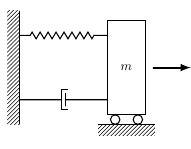
\includegraphics[width=\picwid]{massa_molla_smorzatore_HQ}
 % massa_molla_smorzatore_HQ.png: 0x0 px, 0dpi, 0.00x0.00 cm, bb=
 \label{fig:massa_molla_smorzatore_HQ}
\end{figure}

Si vuole costruire il modello ISU dell'oggetto.
Il corpo ha un solo grado di libertà, si fissa un sistema di riferimento.
Si indica con $s$ la posizione dell'oggetto.

Esistono due modalità principali per scrivere le equazioni di un sistema
meccanico, l'approccio Newtoniano e l'approccio Lagrangiano, si usa in seguito
quello Newtoniano.

Si applica il secondo principio delle dinamica, ossia le formule
precedentemente analizzate.

$$
m\ddot{s} = f - ks - b\dot{s}
$$
$(s_1 , \dot{s}_1 = 0)$

Il numero di equazioni da scrivere è pari al numero di masse moltiplicate per i
rispettivi gradi di libertà.

Le variabili del sistema sono
$$\begin{matrix}
f & s \\
(0) & (2) \\
f & s & \dot{s}\\
u & x_1 &x_2
\end{matrix}$$

Il sistema è del secondo ordine.
$$\left\{\begin{aligned}
\dot{x}_1 &= \dot{s} = x_2 \\
\dot{x}_2 &= \ddot{s} = \frac{1}{m}f - \frac{k}{m}s - \frac{b}{m}s =
-\frac{k}{m}x_1 - \frac{b}{m}x_2 + \frac{1}{m}u
\end{aligned}\right.$$

Le uscite saranno assegnate arbitrariamente, il sistema è lineare
tempo invariante e strettamente causale.












